%% abtex2-modelo-artigo.tex, v-1.9.6 laurocesar
%% Copyright 2012-2016 by abnTeX2 group at http://www.abntex.net.br/ 
%%
%% This work may be distributed and/or modified under the
%% conditions of the LaTeX Project Public License, either version 1.3
%% of this license or (at your option) any later version.
%% The latest version of this license is in
%%   http://www.latex-project.org/lppl.txt
%% and version 1.3 or later is part of all distributions of LaTeX
%% version 2005/12/01 or later.
%%
%% This work has the LPPL maintenance status `maintained'.
%% 
%% The Current Maintainer of this work is the abnTeX2 team, led
%% by Lauro César Araujo. Further information are available on 
%% http://www.abntex.net.br/
%%
%% This work consists of the files abntex2-modelo-artigo.tex and
%% abntex2-modelo-references.bib
%%

% ------------------------------------------------------------------------
% ------------------------------------------------------------------------
% abnTeX2: Modelo de Artigo Acadêmico em conformidade com
% ABNT NBR 6022:2003: Informação e documentação - Artigo em publicação 
% periódica científica impressa - Apresentação
% ------------------------------------------------------------------------
% ------------------------------------------------------------------------

\documentclass[
    % -- opções da classe memoir --
    article,            % indica que é um artigo acadêmico
    11pt,               % tamanho da fonte
    oneside,            % para impressão apenas no recto. Oposto a twoside
    a4paper,            % tamanho do papel. 
    % -- opções da classe abntex2 --
    %chapter=TITLE,     % títulos de capítulos convertidos em letras maiúsculas
    %section=TITLE,     % títulos de seções convertidos em letras maiúsculas
    %subsection=TITLE,  % títulos de subseções convertidos em letras maiúsculas
    %subsubsection=TITLE % títulos de subsubseções convertidos em letras maiúsculas
    % -- opções do pacote babel --
    english,            % idioma adicional para hifenização
    brazil,             % o último idioma é o principal do documento
    sumario=tradicional,
    ]{abntex2}


% ---
% PACOTES
% ---
\usepackage[table,xcdraw]{xcolor}

% ---
% Pacotes fundamentais 
% ---
\usepackage{lmodern}            % Usa a fonte Latin Modern
\usepackage[T1]{fontenc}        % Selecao de codigos de fonte.
\usepackage[utf8]{inputenc}     % Codificacao do documento (conversão automática dos acentos)
\usepackage{indentfirst}        % Indenta o primeiro parágrafo de cada seção.
\usepackage{nomencl}            % Lista de simbolos
\usepackage{color}              % Controle das cores
\usepackage{graphicx}           % Inclusão de gráficos
\usepackage{microtype}          % para melhorias de justificação
% ---
        
% ---
% Pacotes adicionais, usados apenas no âmbito do Modelo Canônico do abnteX2
% ---
\usepackage{lipsum}             % para geração de dummy text
\usepackage{fancyvrb}
\usepackage{todonotes}
\usepackage{float}

% ---
        
% ---
% Pacotes de citações
% ---
\usepackage[brazilian,hyperpageref]{backref}     % Paginas com as citações na bibl
\usepackage[alf]{abntex2cite}   % Citações padrão ABNT
% ---

% ---
% Configurações do pacote backref
% Usado sem a opção hyperpageref de backref
\renewcommand{\backrefpagesname}{Citado na(s) página(s):~}
% Texto padrão antes do número das páginas
\renewcommand{\backref}{}
% Define os textos da citação
\renewcommand*{\backrefalt}[4]{
    \ifcase #1 %
        Nenhuma citação no texto.%
    \or
        Citado na página #2.%
    \else
        Citado #1 vezes nas páginas #2.%
    \fi}%
% ---

% ---
% Informações de dados para CAPA e FOLHA DE ROSTO
% ---
\titulo{INE5644 - Data Mining\\ 
        Exercício Clustering}
\autor{Bruno Marques do Nascimento\thanks{brunomn95@gmail.com \hspace{1mm} - \hspace{1mm} Universidade Federal de Santa Catarina}}
\instituicao{Universidade Federal de Santa Catarina}
\local{Florianópolis - SC, Brasil}
\data{03 de Abril de 2018}
% ---

% ---
% Configurações de aparência do PDF final

% alterando o aspecto da cor azul
\definecolor{blue}{RGB}{41,5,195}

% informações do PDF
\makeatletter
\hypersetup{
        %pagebackref=true,
        pdftitle={\@title}, 
        pdfauthor={\@author},
        pdfsubject={Modelo de artigo científico com abnTeX2},
        pdfcreator={LaTeX with abnTeX2},
        pdfkeywords={abnt}{latex}{abntex}{abntex2}{atigo científico}, 
        colorlinks=true,            % false: boxed links; true: colored links
        linkcolor=blue,             % color of internal links
        citecolor=blue,             % color of links to bibliography
        filecolor=magenta,              % color of file links
        urlcolor=blue,
        bookmarksdepth=4
}
\makeatother
% --- 

% ---
% compila o indice
% ---
\makeindex
% ---

% ---
% Altera as margens padrões
% ---
\setlrmarginsandblock{3cm}{3cm}{*}
\setulmarginsandblock{3cm}{3cm}{*}
\checkandfixthelayout
% ---

% --- 
% Espaçamentos entre linhas e parágrafos 
% --- 

% O tamanho do parágrafo é dado por:
\setlength{\parindent}{1.3cm}

% Controle do espaçamento entre um parágrafo e outro:
\setlength{\parskip}{0.2cm}  % tente também \onelineskip

% Espaçamento simples
\SingleSpacing

% ----
% Início do documento
% ----
\begin{document}

% Seleciona o idioma do documento (conforme pacotes do babel)
%\selectlanguage{english}
\selectlanguage{brazil}

% Retira espaço extra obsoleto entre as frases.
\frenchspacing 

% ----------------------------------------------------------
% ELEMENTOS PRÉ-TEXTUAIS
% ----------------------------------------------------------

%---
%
% Se desejar escrever o artigo em duas colunas, descomente a linha abaixo
% e a linha com o texto ``FIM DE ARTIGO EM DUAS COLUNAS''.
% \twocolumn[           % INICIO DE ARTIGO EM DUAS COLUNAS
%
%---
% página de titulo

\maketitle


% ----------------------------------------------------------
% ELEMENTOS TEXTUAIS
% ----------------------------------------------------------
\textual

% ----------------------------------------------------------
% Introdução
% ----------------------------------------------------------
% \section*{Introdução}
% \addcontentsline{toc}{section}{Introdução}

\section*{\textbf{Respostas:}}
\addcontentsline{toc}{section}{Questões e respostas:}


% ----------------------------------------------------------
% Questão 3
% ----------------------------------------------------------
\subsection*{\textbf{Exercício 3:}}
\addcontentsline{toc}{subsection}{Exercício 3}

\begin{itemize}
    \item{Passo 1:}
        \begin{table}[H]
        \centering
        \label{my-label}
        \begin{tabular}{|l|l|l|l|l|}
        \hline
                   & \textbf{A} & \textbf{B}                        & \textbf{C} & \textbf{D} \\ \hline
        \textbf{B} & 4          &                                   &            &            \\ \hline
        \textbf{C} & 6          & {\color[HTML]{FE0000} \textbf{2}} &            &            \\ \hline
        \textbf{D} & 6          & 4                                 & 2          &            \\ \hline
        \textbf{E} & 7          & 3                                 & 3          & 5          \\ \hline
        \end{tabular}
        \end{table}
    
    \item{Passo 2:}
        \begin{table}[H]
        \centering
        \label{my-label}
        \begin{tabular}{|l|l|l|l|}
        \hline
                    & \textbf{A}               & \textbf{BC}                       & \textbf{D} \\ \hline
        \textbf{BC} & {\color[HTML]{333333} 6} &                                   &            \\ \hline
        \textbf{D}  & 6                        & 4                                 &            \\ \hline
        \textbf{E}  & 7                        & {\color[HTML]{FE0000} \textbf{3}} & 5          \\ \hline
        \end{tabular}
        \end{table}

    \item{Passo 3:}
        \begin{table}[h]
        \centering
        \label{my-label}
        \begin{tabular}{|l|l|l|}
        \hline
                     & \textbf{A} & \textbf{BCE}                      \\ \hline
        \textbf{BCE} & 7          &                                   \\ \hline
        \textbf{D}   & 6          & {\color[HTML]{FE0000} \textbf{5}} \\ \hline
        \end{tabular}
        \end{table}

    \item{Passo 4:}
        \begin{table}[h]
        \centering
        \label{my-label}
        \begin{tabular}{|l|l|}
        \hline
                      & \textbf{A}                        \\ \hline
        \textbf{BCED} & {\color[HTML]{FE0000} \textbf{7}} \\ \hline
        \end{tabular}
        \end{table}

    \item{Resumo:}
        \begin{table}[H]
        \centering
        \label{my-label}
        \begin{tabular}{|l|l|l|}
        \hline
        \textbf{Nó}         & \textbf{Fusão} & \textbf{Nível} \\ \hline
        \textbf{1} & B e C          & 2              \\ \hline
        \textbf{2} & BC e E         & 3              \\ \hline
        \textbf{3} & BCE e D        & 6              \\ \hline
        \textbf{4} & BCED e A       & 7              \\ \hline
        \end{tabular}
        \end{table}
    \item{Dendograma:}
        \begin{figure}[H]
        \label{fig_dendograma1}
        \begin{center}
            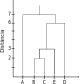
\includegraphics[scale=0.7]{imgs/dendograma1.pdf}
        \end{center}
        \end{figure}
\end{itemize}


\subsection*{\textbf{Exercício 4:}}
\addcontentsline{toc}{subsection}{Exercício 4}

Analisando o dendograma em questão, deveriam ser utilizados 3 \textit{clusters}. Pois, podemos analisar que esse agrupamento se forma em uma região do dendograma que é bem baixa, o que significa que os elementos agrupados nos \textit{clusters} são bem similares, e estes \textit{clusters} só se unirão para formar \textit{clusters} maiores em uma região muito acima, ou seja, a similaridade dos elementos já não será tão alta. 

\subsection*{\textbf{Exercício 5:}}
\addcontentsline{toc}{subsection}{Exercício 5}

\subsubsection*{\textbf{1) minPoints=2 e Eps=3:}}
\addcontentsline{toc}{subsubsection}{Exercício 5.1}

\textbf{Noise:}  X\textsubscript{1}, X\textsubscript{7}, X\textsubscript{5}.

\textbf{Border:} X\textsubscript{9}, X\textsubscript{8}, X\textsubscript{6}.

\textbf{Core:} X\textsubscript{4}, X\textsubscript{2}, X\textsubscript{3}.

\subsubsection*{\textbf{2) minPoints=2 e Eps=4:}}
\addcontentsline{toc}{subsubsection}{Exercício 5.2}

\textbf{Noise:} X\textsubscript{5}.
    
\textbf{Border:} X\textsubscript{9}, X\textsubscript{6}.

\textbf{Core:} X\textsubscript{4}, X\textsubscript{2}, X\textsubscript{3}, X\textsubscript{1}, X\textsubscript{7}, X\textsubscript{8}.
% Finaliza a parte no bookmark do PDF, para que se inicie o bookmark na raiz
% ---
\bookmarksetup{startatroot}% 
% ---

% ---
% Conclusão
% ---
% \section*{Considerações finais}
% \addcontentsline{toc}{section}{Considerações finais}

% ----------------------------------------------------------
% ELEMENTOS PÓS-TEXTUAIS
% ----------------------------------------------------------
\postextual

% ----------------------------------------------------------
% Referências bibliográficas
% ----------------------------------------------------------
\nocite{slides}
\bibliography{bibliography}

\end{document}